\chapter{Whole-Part}

\section{Summary}
Das Whole-Part Design Pattern hilft bei Zusammenführung von Komponenten zu einer logischen Einheit. Dabei wird die ganze Einheit als \textit{Whole} bezeichnet und die einzelnen Teile als \textit{Part}. Das Whole koordiniert die Zusammenarbeit der Parts und bietet ein Interface für alles. Direkter Zugriff auf die Parts ist nicht möglich.
\section{Context}
Implementierung von zusammengesetzten Objekten.
\section{Problem}
Gegeben ist ein komplexes Objekt. Nun soll dieses entweder in kleinere Teilobjekte zerteilt, oder aus weiteren Objekten zu einem ganzen verbunden werden. Clients sollten das Objekt als eine Einheit sehen, welche keinen direkten Zugriff auf die Einzelteile bietet.
\section{Solution}
Es wird mittels des Whole-Part Pattern eine Komponente eingeführt welche die kleineren Objekte in sich kapselt. Diese Komponente definiert ausserdem ein Interface für den Zugriff auf seine Funktionen, und verhindert den direkten Zugriff auf die Einzelteile.  \\
Die Beziehung zwischen Whole und Part kann drei verschiedene Ausprägungen haben:
\begin{enumerate}
	\item \textit{assembly-parts:} Alle Teile sind Eng integriert. Die Anzahl und Art der Teile ist vordefiniert und ändert sich nicht.
	\item \textit{container-contents:} Die Teile sind nicht so Eng gekuppelt wie beim assembly-parts. Es können dynamisch Teile hinzugefügt oder entfernt werden.
	\item \textit{collection-members:} Die Collection gruppiert ähnliche Teile. Es wird kein Unterschied zwischen den einzelnen Teilen gemacht, alle werden gleich behandelt.
\end{enumerate}
\subsection{Structure}
Beim Whole-Part Pattern gibt es zwei Arten von Teilnehmern.
Ein \textit{Whole} Objekt repäsentiert eine Sammlung kleinerer Objekte, welche man  \textit{Part} nennt. Über ein Interface bietet ein Whole eigene Funktionen, sowie die einzelner Parts an. Die folgende Grafik illustriert dieses Zusammenspiel nochmals:
\begin{figure}[H]
	\centering
	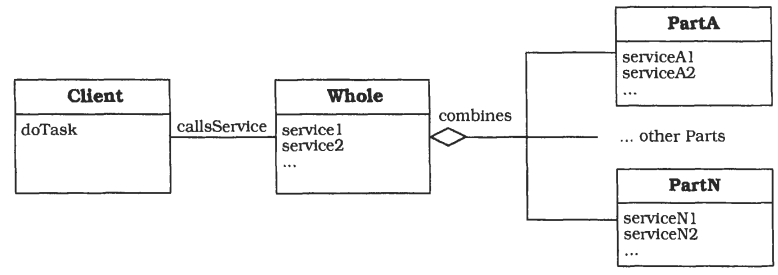
\includegraphics[width=0.7\textwidth]{figures/07-wholepart-1}
	\caption{Whole-Part Zusammenspiel}
\end{figure}

\section{Consequences}
\begin{itemize}
    \pro{bla}
    \con{bla}
\end{itemize}

\section{Known Uses}
\begin{itemize}
	\item Bla
\end{itemize}

\section{Relationships}
\begin{itemize}
	\item \textit{Bla}
\end{itemize}

\section{Exam Questions}
\begin{itemize}
  \item Behauptung: dies ist eine Behauptung? (Lösung)
    \item Frage: Dies ist eine Frage? (Lösung)
\end{itemize}
